\documentclass[11pt]{article}
\usepackage[a4paper, total={6.8in, 9.25in}]{geometry}
\usepackage{graphicx}
\graphicspath{ {./assets/images/output/} }
\usepackage{caption}
\usepackage[english]{babel}
\usepackage{titling}
\usepackage{float}
\usepackage{amsmath}
\usepackage{algorithm}
\usepackage{algorithmicx}
\usepackage{algpseudocode}
\usepackage{minted}
\usepackage{multicol}
\usepackage{array}
\usepackage{setspace}
\usepackage{placeins}
\usepackage{tcolorbox}
\usepackage{caption}
\usepackage{subcaption}

\definecolor{verbgray}{gray}{.95}
\setminted{
    bgcolor=verbgray,
    baselinestretch=1,
    fontsize=\footnotesize,
    linenos,
    breaklines=true,
    breakanywhere=true,
    xleftmargin=\parindent
}
\title{Implementation \& Evaluation of Multi-Class Support Vector Machine (SVM) and Gaussian Naive Bayes}
\author{}
\date{}

\pagenumbering{gobble}
\begin{document}
\input{ml_cover.tex}

\pagebreak

\tableofcontents

\pagebreak
\pagenumbering{arabic}
\maketitle

\section{Theory and Introduction}
This experiment explores two distinct approaches to multi-class classification: the Support Vector Machine (a discriminative, geometric maximum-margin classifier) and Gaussian Naive Bayes (a generative, probabilistic classifier). Both algorithms were implemented from scratch to evaluate their underlying mathematics and decision boundaries.

\subsection{Support Vector Machine (SVM)}
The Support Vector Machine (SVM) maps training examples to points in space to maximize the width of the gap between different categories \cite{bishop2006pattern}. Figure \ref{fig:svm_theory} illustrates the core components of this architecture, highlighting the optimal decision boundary, the maximized margin, and the critical support vectors that anchor the boundary.

\begin{figure}[H]
    \centering
    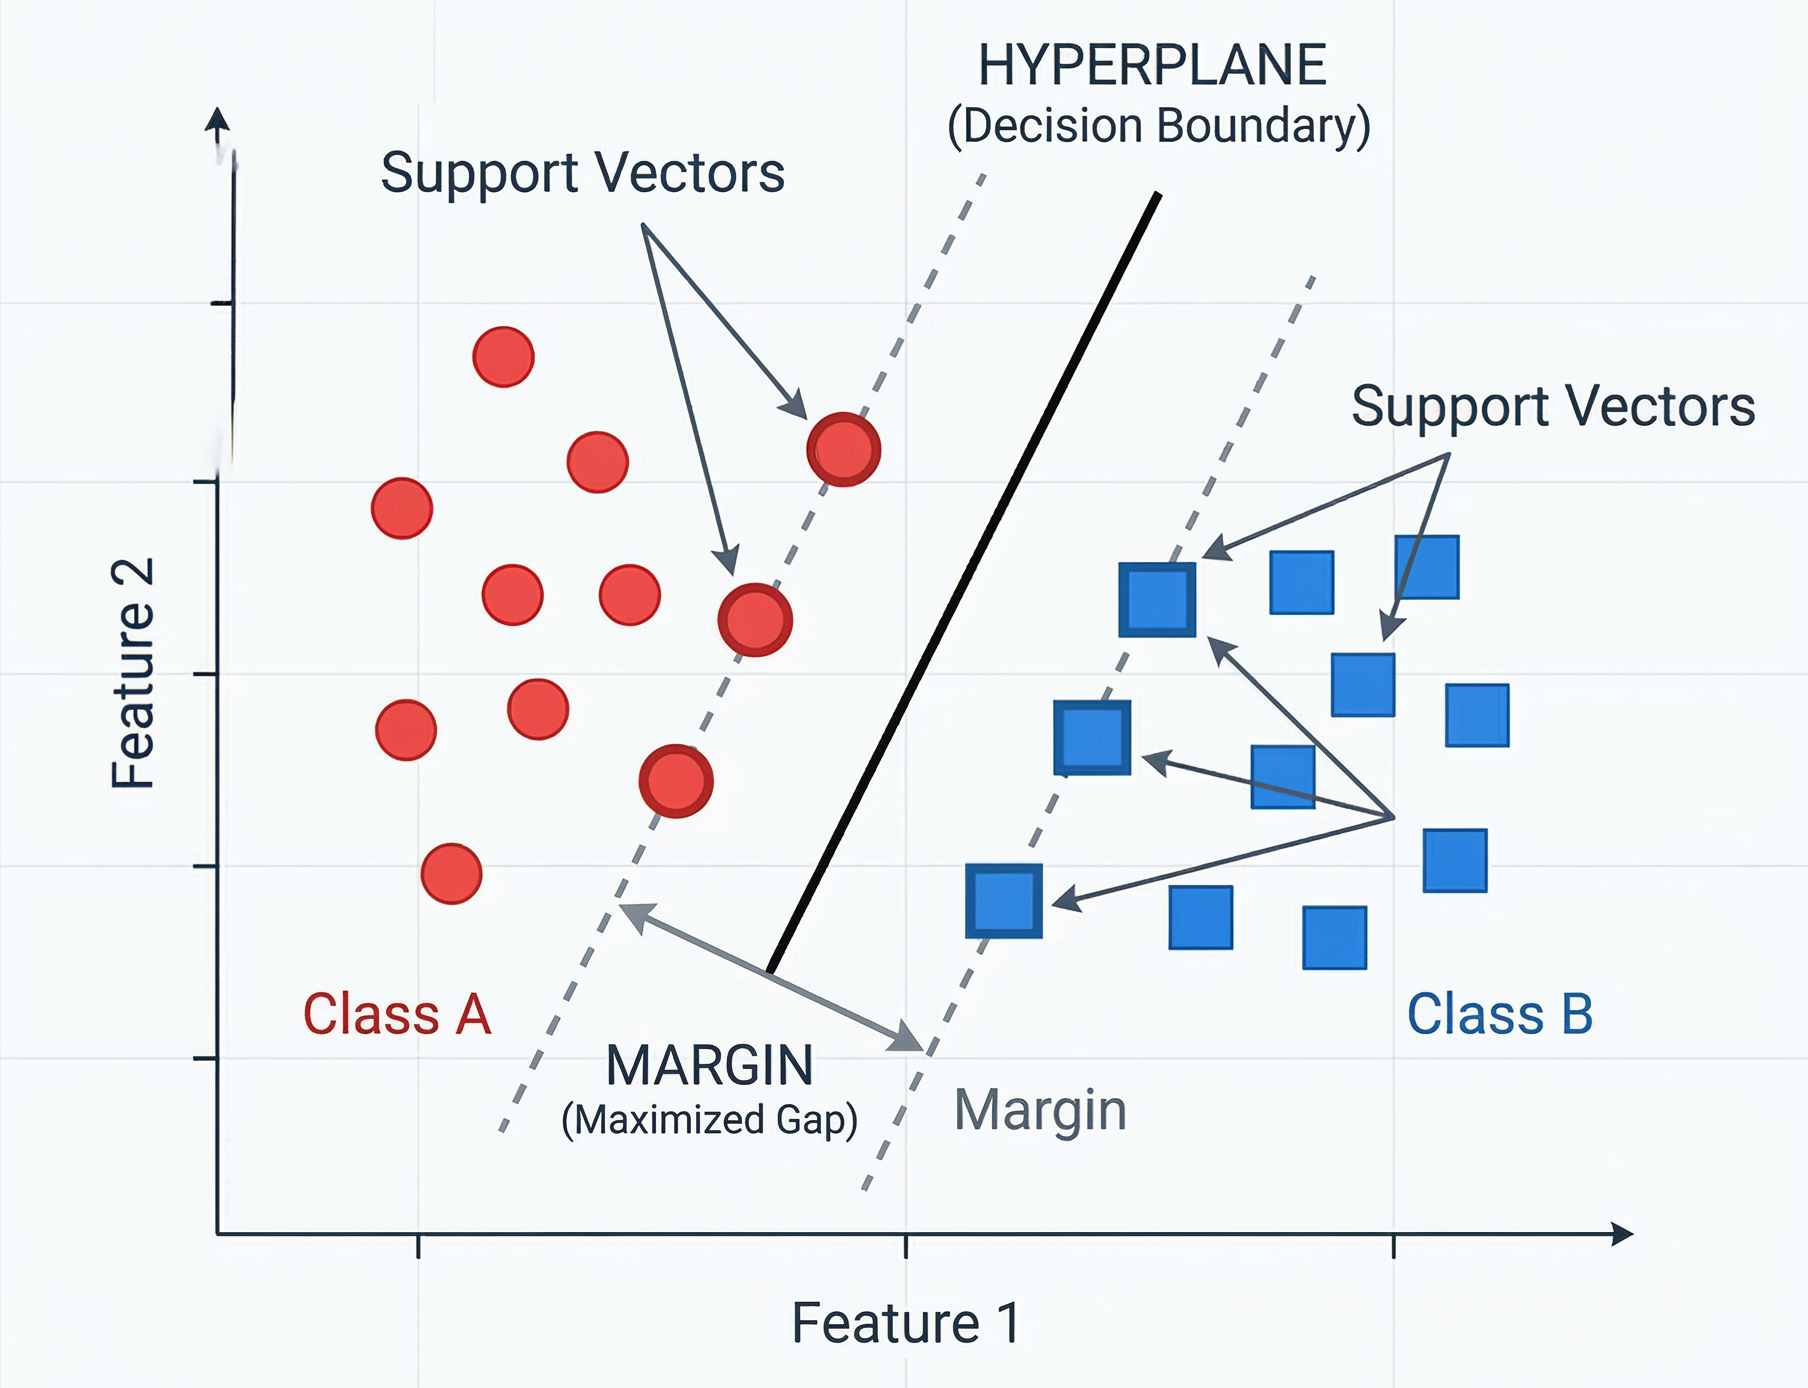
\includegraphics[width=0.37\textwidth]{svm.png}
    \caption{Conceptual illustration of a binary Support Vector Machine. The algorithm identifies the optimal hyperplane that maximizes the margin gap between Class A and Class B. The data points lying directly on the margin boundaries are the support vectors.}
    \label{fig:svm_theory}
\end{figure}

For a binary classification task where labels $y \in \{-1, 1\}$, a linear SVM minimizes the Hinge Loss with $L_2$ regularization:
\begin{equation}
    J(w, b) = \lambda ||w||^2 + \frac{1}{n} \sum_{i=1}^{n} \max(0, 1 - y_i(w^T x_i + b))
\end{equation}
Standard SVMs are strictly binary classifiers. To classify $K$ classes, $K$ separate binary SVM models are trained using the One-vs-Rest (OvR) strategy. For a new input $x$, the class is assigned to the classifier yielding the highest confidence score:
\begin{equation}
    \hat{y} = \arg\max_{k \in \{1, \dots, K\}} (w_k^T x + b_k)
\end{equation}

\subsection{Gaussian Naive Bayes}
Naive Bayes relies on Bayes' Theorem to predict the probability of a class $y_k$ given an input feature vector $X$. It assumes that all features are mutually independent given the class \cite{hastie2009elements}.
\begin{equation}
    P(y_k | X) = \frac{P(y_k) \prod_{i=1}^{n} P(x_i | y_k)}{P(X)}
\end{equation}
For continuous data, it is assumed that the continuous values associated with each class are distributed according to a Gaussian (Normal) distribution. The likelihood $P(x_i | y_k)$ is calculated using the Gaussian Probability Density Function (PDF):
\begin{equation}
    P(x_i | y_k) = \frac{1}{\sqrt{2\pi\sigma_{k,i}^2}} \exp\left(-\frac{(x_i - \mu_{k,i})^2}{2\sigma_{k,i}^2}\right)
\end{equation}
Where $\mu_{k,i}$ and $\sigma_{k,i}^2$ are the mean and variance of feature $i$ in class $k$. To avoid numerical underflow, the log-posterior is maximized during prediction instead of the raw probability product:
\begin{equation}
    \hat{y} = \arg\max_k \left( \log P(y_k) + \sum_{i=1}^{n} \log P(x_i | y_k) \right)
\end{equation}

\section{Methodology}

\subsection{Dataset}
The \textit{Iris} dataset was utilized, containing three distinct classes (\textit{Setosa}, \textit{Versicolor}, and \textit{Virginica}). The dataset was standardized. Two features (Petal Length and Petal Width) were used to allow for 2D visualization of the decision boundaries \cite{fisher1936use}.

\subsection{Algorithms}

\begin{algorithm}[H]
    \caption{Multi-Class SVM (One-vs-Rest Training via SGD)}
    \begin{algorithmic}[1]
        \State \textbf{Input:} Training Data $(X, Y)$ with $K$ classes, $\lambda$, $\alpha$, $epochs$
        \State \textbf{Initialize:} $K$ instances of Binary SVMs
        \For{$k = 1$ to $K$}
        \State $Y_{binary} \gets \{1 \text{ if } y_i == k \text{ else } -1 \text{ for } y_i \in Y\}$
        \State \textbf{Train} Model$_k$ on $(X, Y_{binary})$ using Hinge Loss and SGD
        \EndFor
        \State \Return array of trained models
    \end{algorithmic}
\end{algorithm}

\begin{algorithm}[H]
    \caption{Gaussian Naive Bayes (Training \& Prediction)}
    \begin{algorithmic}[1]
        \Function{Fit}{$X, y$}
        \For{each class $k \in K$}
        \State $\mu_k \gets \text{Mean of } X \text{ where } y = k$
        \State $\sigma^2_k \gets \text{Variance of } X \text{ where } y = k$
        \State $P(y_k) \gets \frac{\text{Count}(y=k)}{\text{Total Samples}}$
        \EndFor
        \EndFunction
        \Function{Predict}{$x_{query}$}
        \For{each class $k \in K$}
        \State $posterior_k \gets \log P(y_k) + \sum \log \left( \text{GaussianPDF}(x_{query}, \mu_k, \sigma^2_k) \right)$
        \EndFor
        \State \Return $\arg\max_k (posterior_k)$
        \EndFunction
    \end{algorithmic}
\end{algorithm}

\subsection{Code}
The algorithms were implemented in Python using NumPy for matrix operations.
\subsubsection*{SVM Implementation}
\begin{multicols}{2}
    \inputminted{python}{./assets/svm_3class.py}
\end{multicols}

\subsubsection*{Naive Bayes Implementation}
\begin{multicols}{2}
    \inputminted{python}{./assets/naive_bayes.py}
\end{multicols}

\section{Results and Discussion}

\subsection{Support Vector Machine Results}
The Multi-Class SVM was trained using $K=3$ binary classifiers with a learning rate of $0.01$, a lambda parameter of $0.01$, over $1500$ epochs.

\begin{minted}{console}
==================================================
 MULTI-CLASS SVM (One-vs-Rest) CLASSIFICATION
==================================================
Loading Iris Dataset...
Training Multi-Class SVM (One-vs-Rest strategy)...
  -> Training SVM 1 (Class 0 vs Rest)...
  -> Training SVM 2 (Class 1 vs Rest)...
  -> Training SVM 3 (Class 2 vs Rest)...

========================================
EVALUATION REPORT (3-Class)
========================================
Accuracy:  0.9333
Precision (Macro): 0.9327
Recall (Macro):    0.9393
F1 Score (Macro):  0.9350

Confusion Matrix:
[[ 7  0  0]
 [ 1  9  1]
 [ 0  0 12]]
\end{minted}

\begin{figure}[H]
    \centering
    \begin{subfigure}[b]{0.45\textwidth}
        \centering
        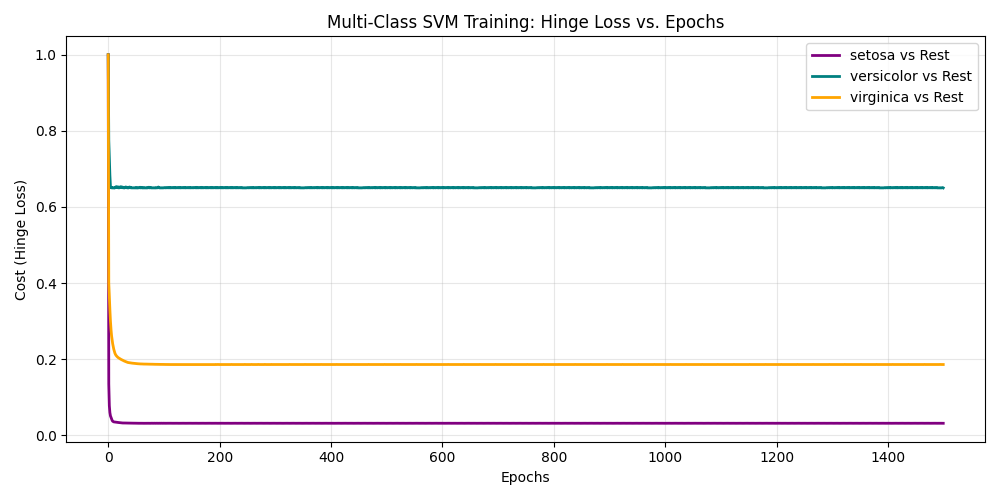
\includegraphics[width=\textwidth]{cost.png}
        \caption{Hinge Loss vs. Epochs}
    \end{subfigure}
    \hfill
    \begin{subfigure}[b]{0.45\textwidth}
        \centering
        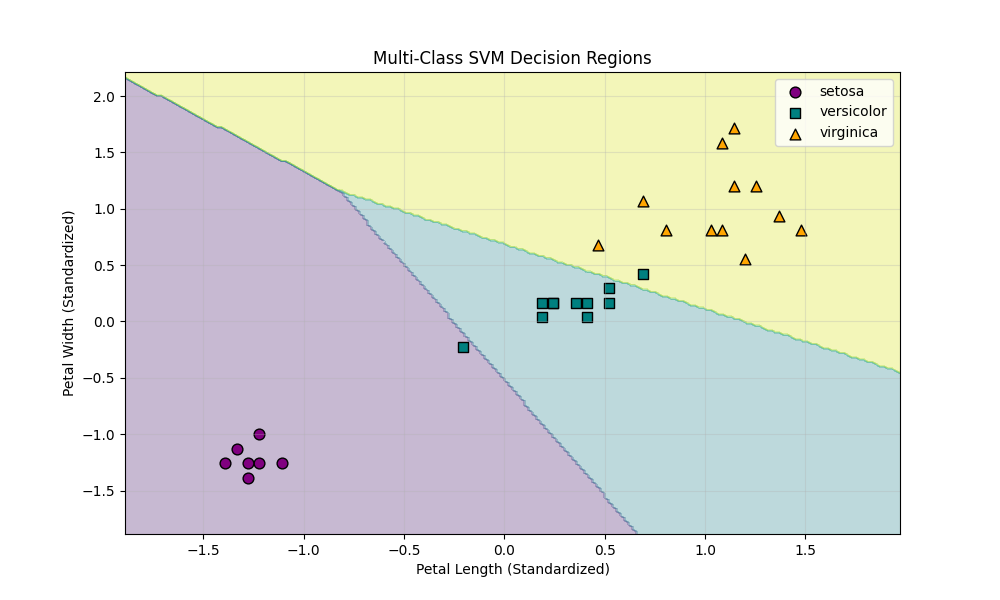
\includegraphics[width=\textwidth]{decision.png}
        \caption{Decision Regions (OvR Boundary)}
    \end{subfigure}

    \vspace{0.5cm}
    \begin{subfigure}[b]{0.45\textwidth}
        \centering
        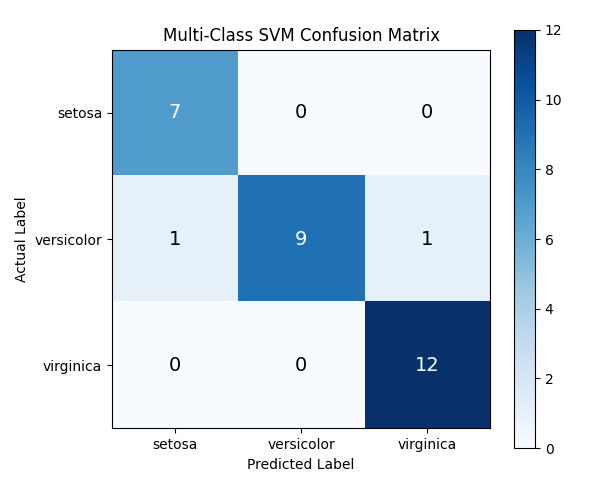
\includegraphics[width=\textwidth]{confusion.png}
        \caption{Multi-Class SVM Confusion Matrix}
    \end{subfigure}
    \caption{Multi-Class SVM Performance Overview}
    \label{fig:svm_results}
\end{figure}

The SVM achieved an accuracy of 93.33\%. The cost function (Figure \ref{fig:svm_results}a) demonstrates distinct convergence behavior. Separating the middle cluster (\textit{Versicolor}) from the extremes yields a higher residual cost compared to the other two classes. The decision boundary (Figure \ref{fig:svm_results}b) reveals the sharp, piecewise linear angles characteristic of the One-vs-Rest geometric approach.

\subsection{Gaussian Naive Bayes Results}
The Gaussian Naive Bayes model was trained by analytically calculating the means and variances of the dataset, requiring zero iterative epochs.

\begin{minted}{console}
==================================================
 GAUSSIAN NAIVE BAYES CLASSIFICATION
==================================================

Training Gaussian Naive Bayes Model...

========================================
EVALUATION REPORT (3-Class)
========================================
Accuracy:  0.9667
Precision (Macro): 0.9722
Recall (Macro):    0.9722
F1 Score (Macro):  0.9722

Confusion Matrix:
[[ 7  0  0]
 [ 0 11  0]
 [ 0  1 11]]
\end{minted}

\begin{figure}[H]
    \centering
    \begin{subfigure}[b]{0.48\textwidth}
        \centering
        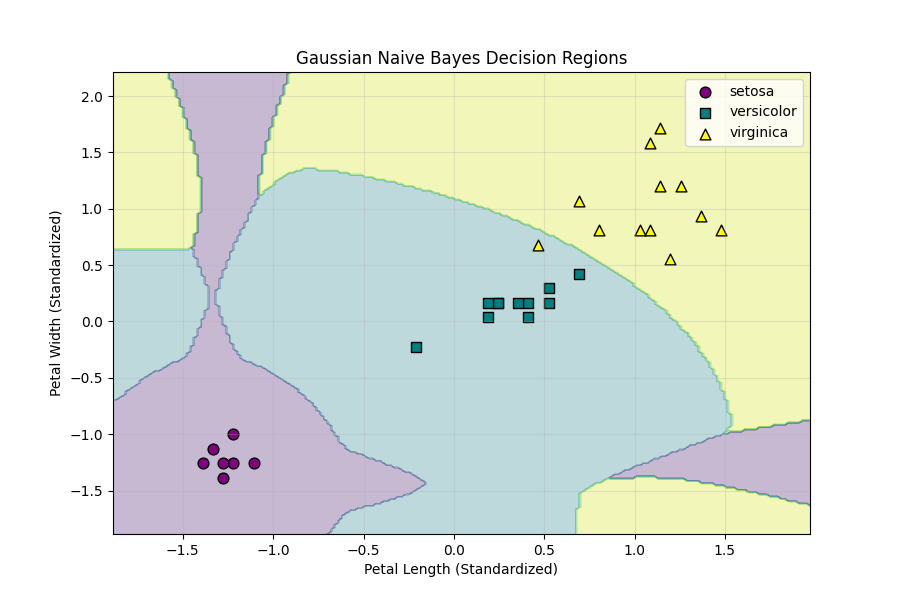
\includegraphics[width=\textwidth]{n_dec.png}
        \caption{Gaussian Naive Bayes Decision Regions}
    \end{subfigure}
    \hfill
    \begin{subfigure}[b]{0.48\textwidth}
        \centering
        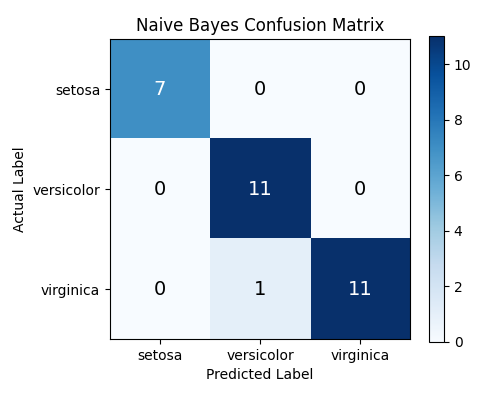
\includegraphics[width=\textwidth]{n_conf.png}
        \caption{Naive Bayes Confusion Matrix}
    \end{subfigure}
    \caption{Gaussian Naive Bayes Performance Overview}
    \label{fig:nb_results}
\end{figure}

The Naive Bayes model outperformed the SVM on this dataset slice, achieving 96.67\% accuracy. The confusion matrix (Figure \ref{fig:nb_results}b) shows only a single misclassification: one \textit{Virginica} sample predicted as \textit{Versicolor}.

In contrast to the strict linear cuts of the SVM, the decision boundary of Naive Bayes (Figure \ref{fig:nb_results}a) features curved (quadratic) lines. Because the covariance matrices between the features are not assumed to be equal, the intersection of their Gaussian probability distributions results in naturally curved boundaries, which better capture the overlapping spread of the \textit{Versicolor} and \textit{Virginica} clusters.

\section{Conclusion}
This experiment successfully demonstrated the contrast between discriminative (SVM) and generative (Naive Bayes) multi-class classification.
\begin{itemize}
    \item \textbf{Support Vector Machine} accurately classified the data (93.33\%) by solving an optimization problem to find maximum-margin hyperplanes. The One-vs-Rest strategy successfully merged these binary models into a rigid, piecewise linear decision space.
    \item \textbf{Gaussian Naive Bayes} achieved superior accuracy (96.67\%) without the need for iterative gradient descent. By modeling the underlying probability distributions of the features, it constructed fluid, quadratic decision boundaries that effectively mapped the overlapping variance of the natural data.
\end{itemize}

\bibliographystyle{IEEEtran}
\renewcommand{\bibname}{References}
\addcontentsline{toc}{section}{References}
\bibliography{ref}

\end{document}